\documentclass[11pt,a4paper,oneside]{report}
\usepackage{amsmath,amssymb,calc,ifthen}
\usepackage{float}
%\usepackage{cancel}
\usepackage[table,usenames,dvipsnames]{xcolor} % for coloured cells in tables
\usepackage{tikz}
% Allows us to click on links and references!
\usepackage{hyperref}
\usepackage{url}
\hypersetup{
colorlinks,
citecolor=black,
filecolor=black,
linkcolor=black,
urlcolor=black
}
% Nice package for plotting graphs
% See excellent guide:
% http://www.tug.org/TUGboat/tb31-1/tb97wright-pgfplots.pdf
\usetikzlibrary{plotmarks,shapes}
\usepackage{amsmath,graphicx}
\usepackage{epstopdf}
\usepackage{caption}
\usepackage{subcaption}
\usepackage{graphicx}
% highlight - useful for TODOs and similar
\usepackage{color}
\newcommand{\hilight}[1]{\colorbox{yellow}{#1}}
\newcommand\ci{\perp\!\!\!\perp} % perpendicular sign
\newcommand*\rfrac[2]{{}^{#1}\!/_{#2}} % diagonal fraction
\newcommand\SLASH{\char`\\}
\usepackage{listings}
% margin size
\usepackage[margin=0.65in]{geometry}
\usepackage{pdfpages}

\usepackage{titlesec} % reduce spacing after subsections

% \titlespacing\subsection{0pt}{4pt plus 4pt minus 2pt}{4pt plus 2pt minus 2pt}


\begin{document}
\belowdisplayskip=12pt plus 3pt minus 9pt
\belowdisplayshortskip=7pt plus 3pt minus 4pt


% \rowcolors{2}{gray!25}{white}




\begin{figure}[H]
\centering
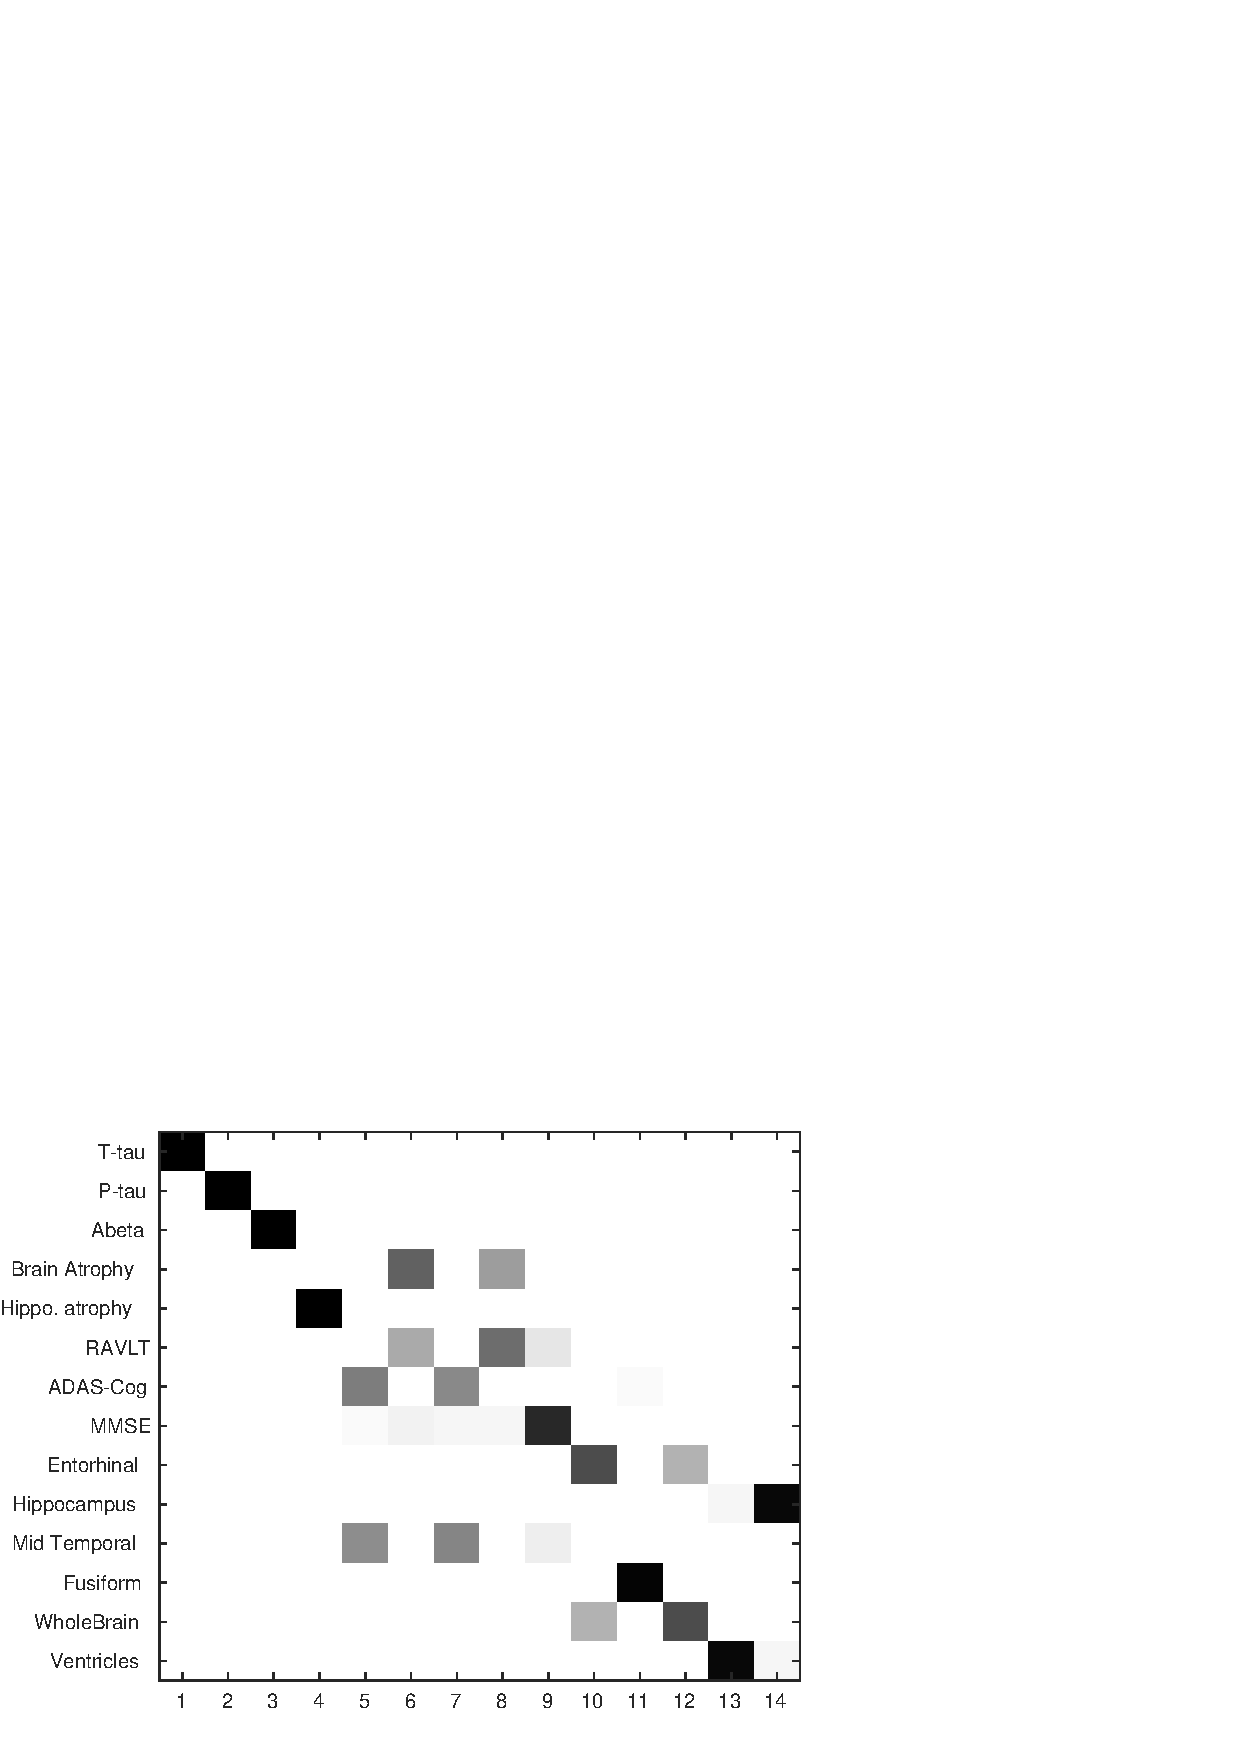
\includegraphics[scale=0.75]{alex_mat_max_like.png}
\caption{Maximum likelihood ordering}
\end{figure}

\begin{figure}[H]
\centering
\includegraphics[scale=0.75]{alex_mat_char_seq.png}
\caption{Characteristic ordering}
\end{figure}

\end{document}





















